\documentclass[draft,handout]{beamer}
\usepackage[orientation=portrait,size=A4]{beamerposter} 

\usepackage[utf8]{inputenc}
\usepackage[T1]{fontenc}
\usepackage[french]{babel}
\usepackage{graphicx}


\newcommand{\ensemble}[1]{\left\lbrace{} #1 \right\rbrace{}}

\usetheme{Boadilla}

\title{Optimisation de circuits logiques}

\author{Alexandre JANNIAUX}

\begin{document}

\begin{frame}
        \maketitle
        \tableofcontents
    \end{frame}

    \begin{frame}{Circuits logiques et fonctions combinatoires}
            \begin{figure}[p]
                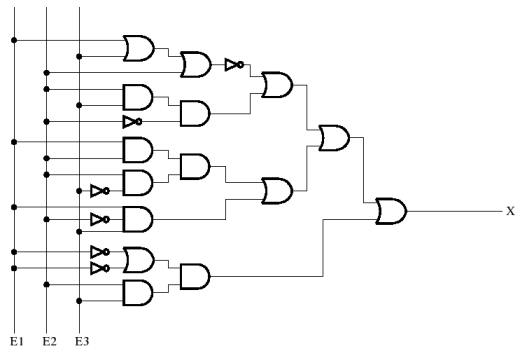
\includegraphics[width=8cm]{images/circuit_logique.png}
                \caption{Exemple de circuit logique}
               \label{fig:circ1}
            \end{figure}

        \[ \begin{aligned}
                f: \ensemble{0,1}^3 &\longto & \ensemble{0,1} \\
                (e_1,e_2,e_3) & \longmapsto & f(e_1,e_2,e_3) 
            \end{aligned}
        \]

        L'ensemble des fonctions combinatoires défini par induction

        MAIS: explosion combinatoire (algo naif)

    \end{frame}

    \begin{frame}{M\'ethode de Quine-McCluskey}

        \large{\textbf{Idée :}} Une fonction combinatoire est définie par le langage accepté (couverture).

        => On utilise l'algèbre de Boole pour simplifier les expressions

        \large{\textbf{Algorithme :}}
            \begin{enumerate}
                \item 
            \end{enumerate}
    \end{frame}

    \begin{frame}
        \frametitle{M\'ethode de Petrick}

    \end{frame}
\end{document}
